\documentclass[tikz,border=5pt]{standalone}
\usepackage{tikz}
\usetikzlibrary{angles,quotes}
\definecolor{nebula}{HTML}{6366F1}
\definecolor{spark}{HTML}{14B8A6}
\definecolor{ink}{HTML}{334155}
\begin{document}
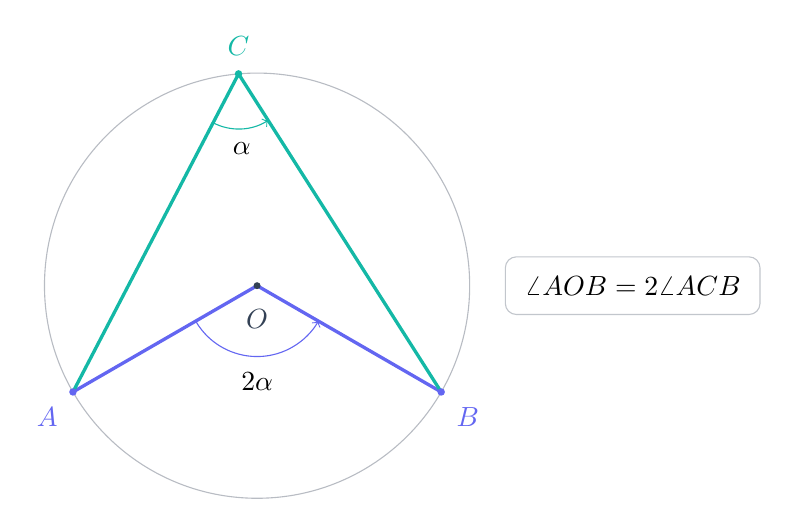
\begin{tikzpicture}[font=\sffamily,scale=.9]
  \coordinate (O) at (0,0);
  \coordinate (A) at (210:3);
  \coordinate (B) at (330:3);
  \coordinate (C) at (95:3);
  \draw[ink!35] (O) circle (3);
  \draw[very thick,nebula] (A)--(O)--(B);
  \draw[very thick,spark] (A)--(C)--(B);
  \fill[ink] (O) circle (1.4pt) node[below=5pt] {$O$};
  \fill[nebula] (A) circle (1.5pt) node[below left=2pt] {$A$};
  \fill[nebula] (B) circle (1.5pt) node[below right=2pt] {$B$};
  \fill[spark] (C) circle (1.5pt) node[above=3pt] {$C$};
  \pic[draw=nebula,->,"$2\alpha$",angle radius=9mm,angle eccentricity=1.35] {angle=A--O--B};
  \pic[draw=spark,->,"$\alpha$",angle radius=7mm,angle eccentricity=1.35] {angle=A--C--B};
  \node[draw=ink!30,rounded corners=4pt,fill=white,inner sep=7pt] at (5.3,0)
    {$\angle AOB=2\angle ACB$};
\end{tikzpicture}
\end{document}
